\section{Results}\label{sec:results}
Unfortunately, there turns out to be a fundamental contradiction that arises
when photometric stereo is attempted on a scene with a single stationary
perfect mirror: the total light vector when both the direct and reflected light
sources are visible to a pixel (the third case in
Equation~\ref{eq:combinations}) is \emph{always} coplanar, which is precisely
the situation in which Equation~\ref{eq:pseudoinverse} is underconstrained, due
to the pseudoinverse losing rank. As a result, none of the proposed approaches
would be capable of producing the correct normal vector, and a depth map could
not be recovered. See Figures~\ref{fig:output-candidates}
and~\ref{fig:output-combined} for a visualization of the output
of the least-squares approach.

To see why this is the case, consider the sum of $\light$ and $\light'$ in
Figure~\ref{fig:light-reflection}. Since $\light$ and $\light'$ always have the
same magnitude in the presense of a perfectly reflective mirror (one by which
light intensity is preserved), the vertical component cancels out and the
resulting vector is always parallel to the mirror plane. This is seen from
Equations~\ref{eq:light-reflection} and~\ref{eq:combinations}:
\begin{equation}
    \tilde{\light}_i = \light_i + \light_i'
                     = 2 \light_i - 2 \light_i^\parallel
                     = 2 \light_i^\perp
\end{equation}
Since the most common light combination is arguably this one in which neither
the direct nor the mirrored light is occluded, especially with shallow incident
light angles on the mirror surface, this is a significant handicap on the
utility of photometric stereo in the presence of such a mirror. Note that this
phenomenon only necessarily applies when the light is directional and the
mirror is stationary (i.e., its position does not vary between frames) and has
high reflectivity.
\begin{figure}
  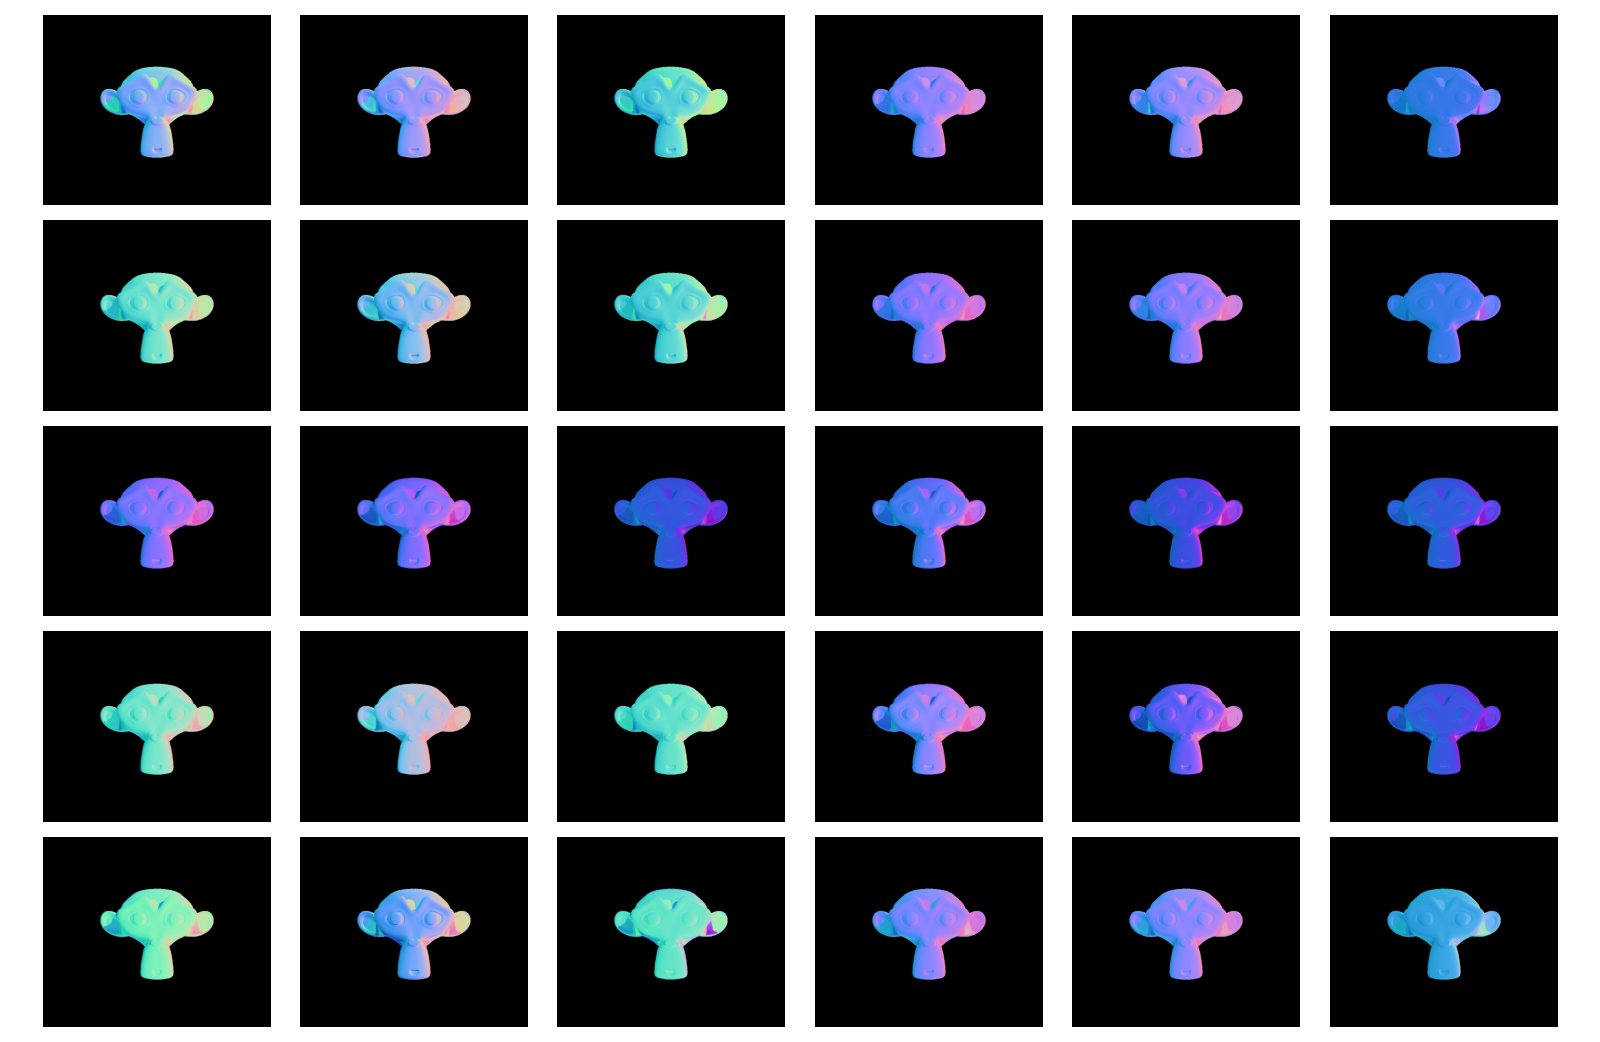
\includegraphics[width=\columnwidth]{images/output-candidates}
  \caption{A visualization of the first 30 of the 243 ($3^N$ with $N = 5$)
  computed normal maps assuming a different combination of light visible to the
  scene in each one. Within each of these candidate maps, the combination of
  lights incident on all pixels is assumed to be the same within a frame.
  Theoretically, the correct normal map can be constructed by selecting the
  correct option for each pixel among the candidates. Due to light source
  coplanarity and the subsequent loss of rank in the light matrix, the last
  such map (the one in which light from both the direct and the mirrored light
  sources is visible) is always blank.}\label{fig:output-candidates}
\end{figure}
\begin{figure}
  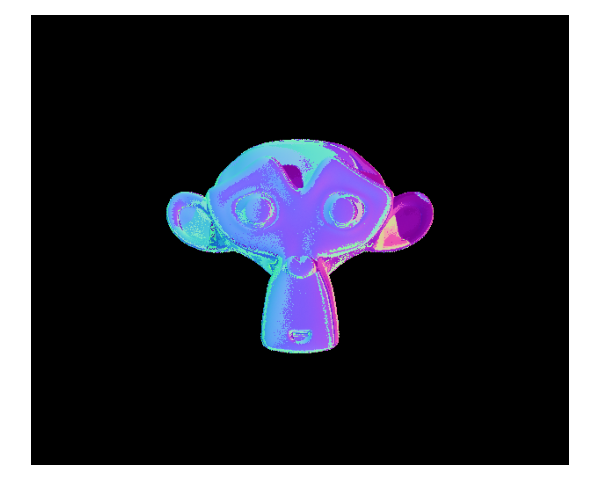
\includegraphics[width=\columnwidth]{images/output-combined}
  \caption{A visualization of the normal map constructed by the least-squares
  approach. Note that the most likely candidate for most pixels in the scene
  (the one in which all both the direct and the mirrored light sources is
  visible to a pixel in every frame) is invalid as described in
  Section~\ref{sec:results}. As a result, most of the obtained values are
  wrong.}\label{fig:output-combined}
\end{figure}

